\documentclass{article}

\usepackage[english]{babel}
\usepackage[utf8]{inputenc}
\usepackage{amsmath,amssymb}
\usepackage{parskip}
\usepackage{graphicx}
\usepackage{listings}
\usepackage{float}
\usepackage{subfig}



\lstset{ %
language=python,                % the language of the code
basicstyle=\footnotesize,           % the size of the fonts that are used for the code
numbers=left,                   % where to put the line-numbers
numberstyle=\tiny\color{gray},  % the style that is used for the line-numbers
stepnumber=2,                   % the step between two line-numbers. If it's 1, each line 
                                % will be numbered
numbersep=5pt,                  % how far the line-numbers are from the code
backgroundcolor=\color{white},      % choose the background color. You must add \usepackage{color}
showspaces=false,               % show spaces adding particular underscores
showstringspaces=false,         % underline spaces within strings
showtabs=false,                 % show tabs within strings adding particular underscores
frame=single,                   % adds a frame around the code
rulecolor=\color{black},        % if not set, the frame-color may be changed on line-breaks within not-black text (e.g. commens (green here))
tabsize=2,                      % sets default tabsize to 2 spaces
captionpos=b,                   % sets the caption-position to bottom
breaklines=true,                % sets automatic line breaking
breakatwhitespace=false,        % sets if automatic breaks should only happen at whitespace
title=\lstname,                 % show the filename of files included with \lstinputlisting;
                                % also try caption instead of title
keywordstyle=\color{blue},          % keyword style
commentstyle=\color{dkgreen},       % comment style
stringstyle=\color{mauve},         % string literal style
escapeinside={\%*}{*)},            % if you want to add LaTeX within your code
morekeywords={*,...}               % if you want to add more keywords to the set
}
% Margins
\usepackage[top=2.5cm, left=3cm, right=3cm, bottom=4.0cm]{geometry}
% Colour table cells
\usepackage[table]{xcolor}

% Get larger line spacing in table
\newcommand{\tablespace}{\\[1.25mm]}
\newcommand\Tstrut{\rule{0pt}{2.6ex}}         % = `top' strut
\newcommand\tstrut{\rule{0pt}{2.0ex}}         % = `top' strut
\newcommand\Bstrut{\rule[-0.9ex]{0pt}{0pt}}   % = `bottom' strut

%%%%%%%%%%%%%%%%%
%     Title     %
%%%%%%%%%%%%%%%%%
\title{CSCI803 Assignment}
\author{Yao Xiao \\ SID 2019180015}
\date{\today}

\begin{document}
\maketitle

%%%%%%%%%%%%%%%%%
%   Problem 1   %
%%%%%%%%%%%%%%%%%
\section{Problem 1}
AVL tree:
An AVL tree is a self-balancing binary search tree, balanced to maintain $O(lgn)$ height.
And it is usually used for in memory backed search trees.

B-tree:
A B-tree is a balanced tree, but it is not a binary tree. Nodes have more children, which increases per-node search time but decreases the number of nodes the search needs to visit.
And it is rimarily used as a storage backed search tree for very large datasets because it requires less reads to disk (since each node contains N keys where N>1). 

\section{Problem 2}

\begin{figure}[H]
    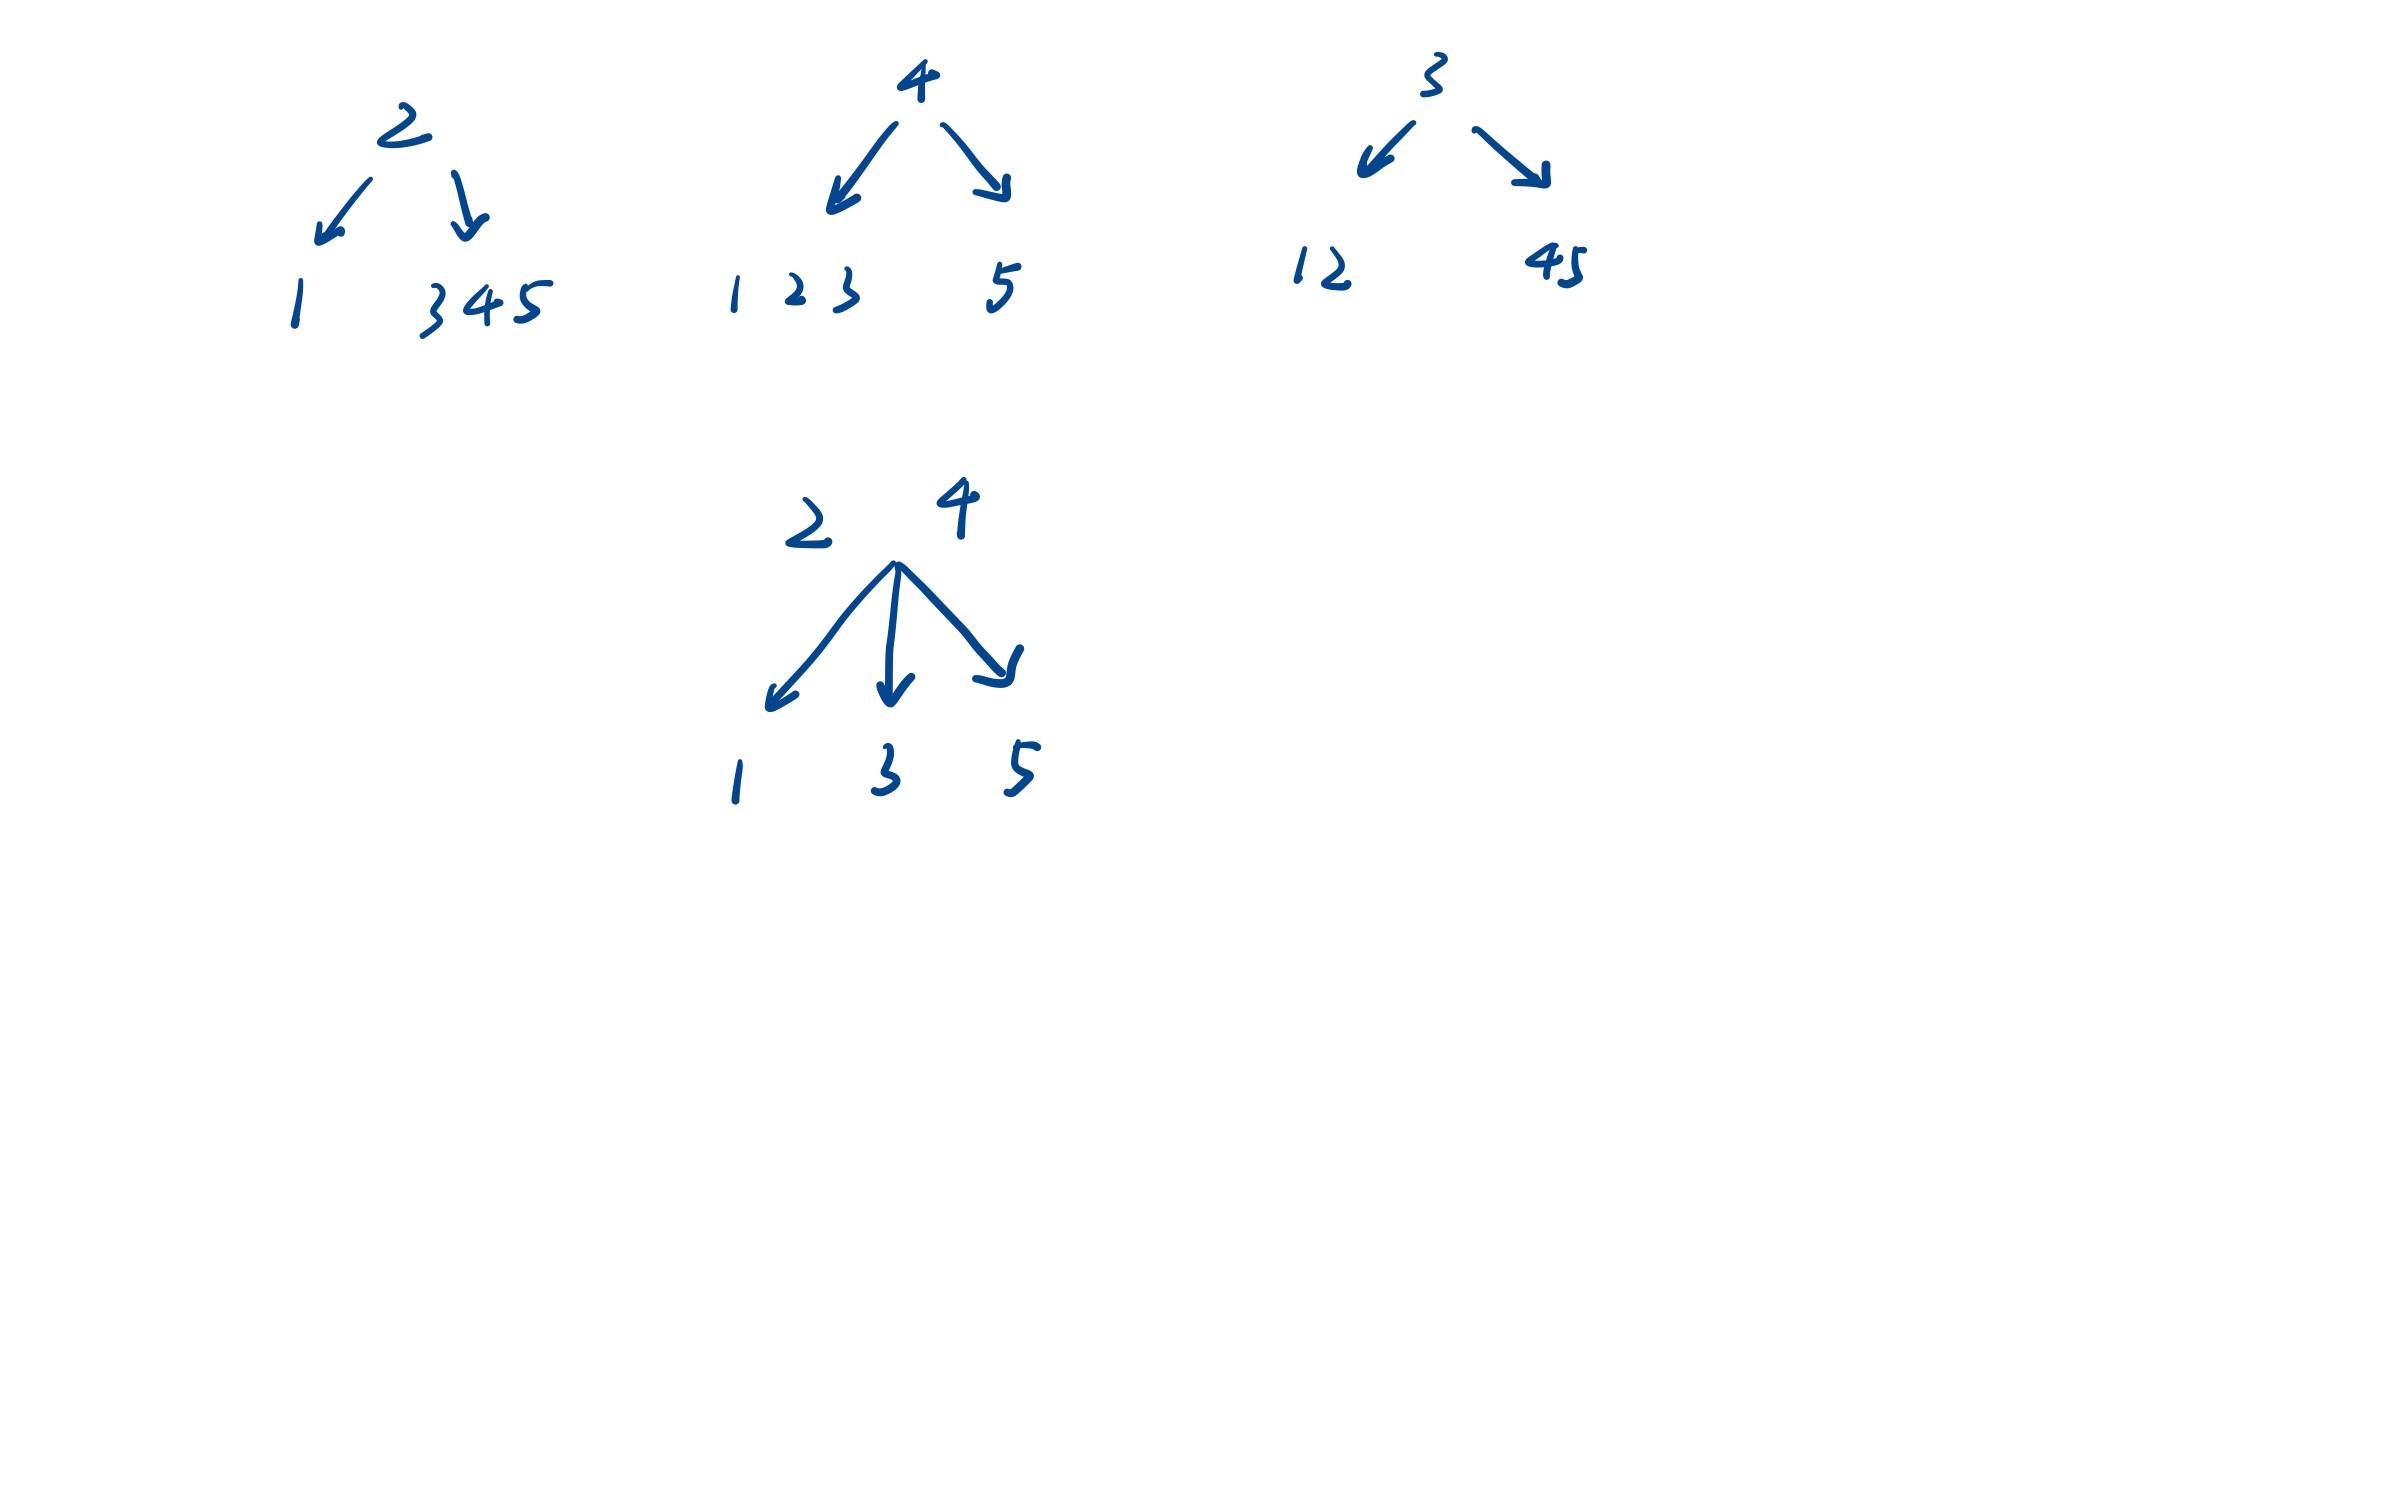
\includegraphics[width=1\textwidth]{Fig1}
\end{figure}

\section{Problem 3}
\begin{figure}[H]
    \subfloat{
        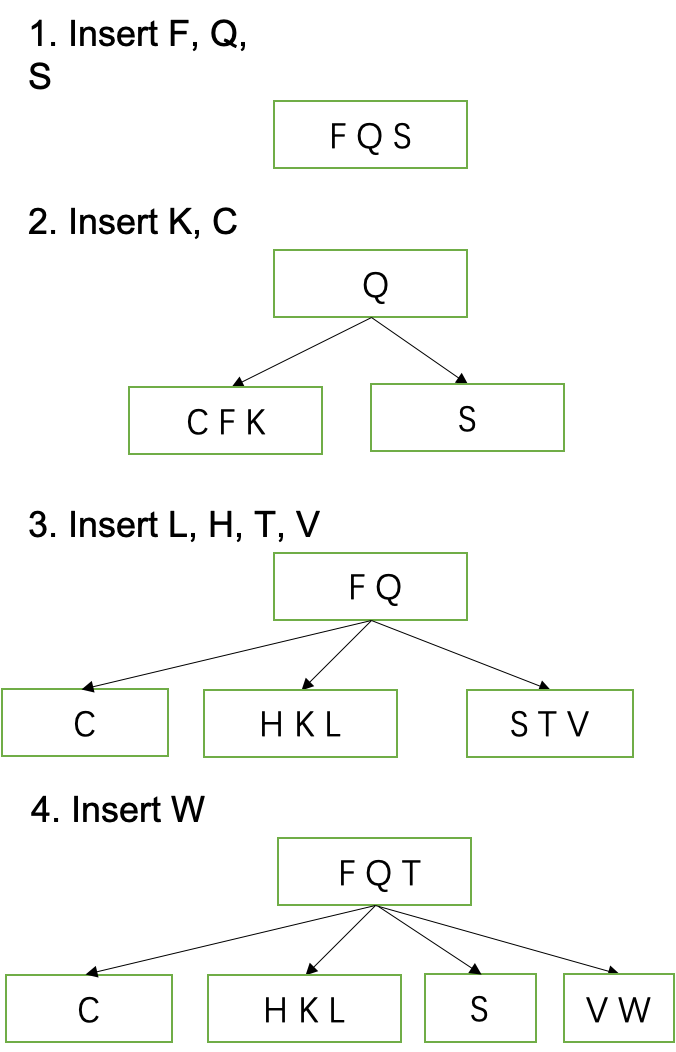
\includegraphics[width=0.5\textwidth]{Fig2}
    }
\end{figure}
\begin{figure}[H]
    \subfloat{
        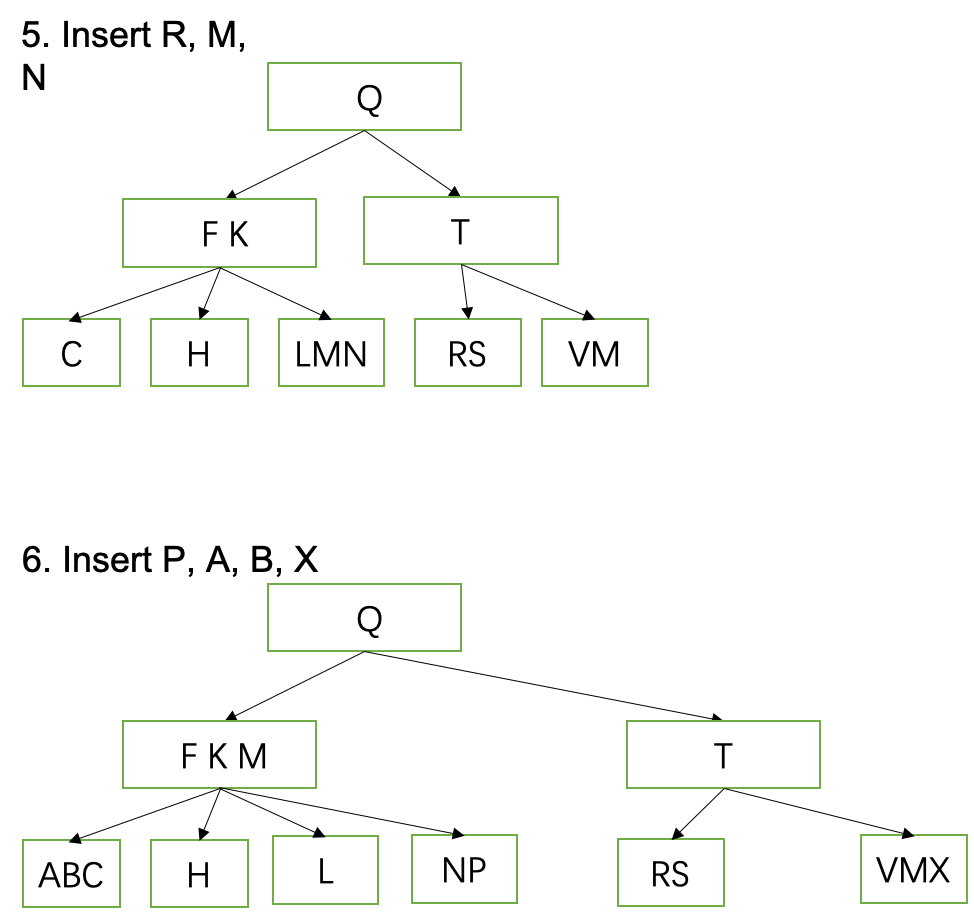
\includegraphics[width=0.7\textwidth]{Fig3}
    }
\end{figure}
\begin{figure}[H]
    \subfloat{
        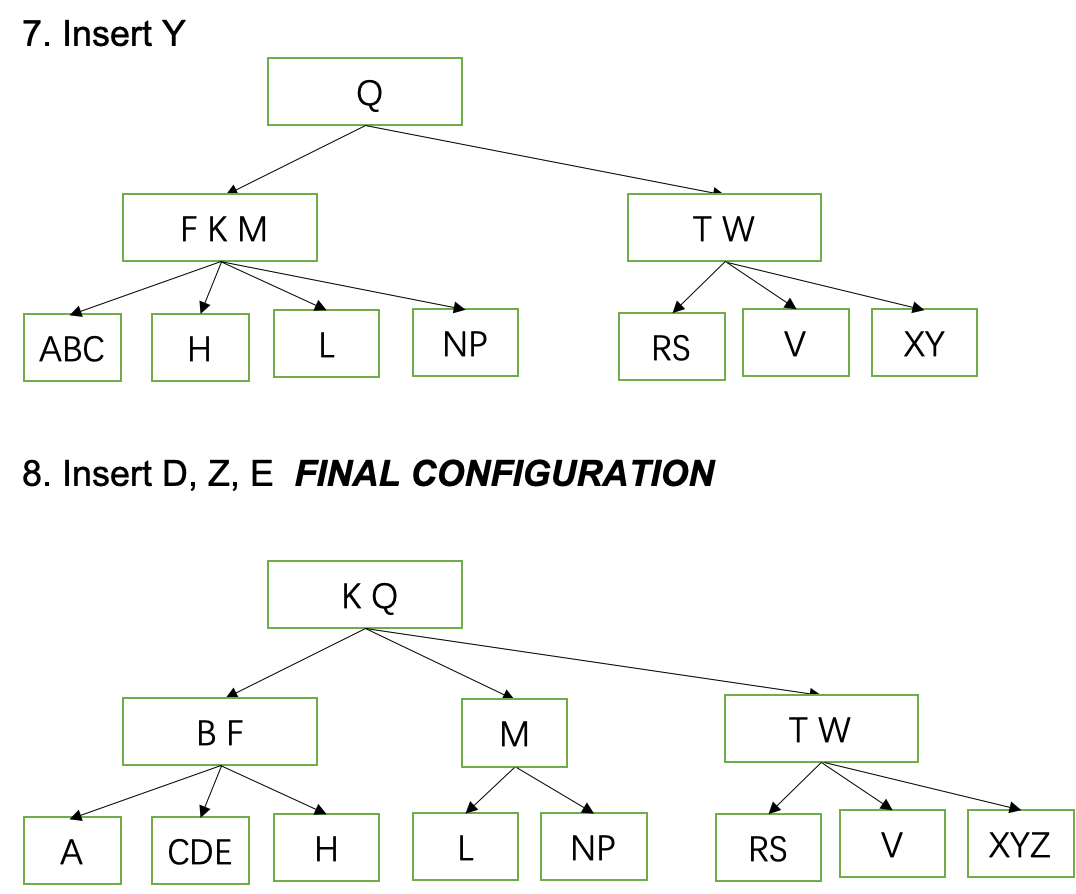
\includegraphics[width=0.7\textwidth]{Fig4}
    }
\end{figure}


\end{document}
